\chapter{Improved tolopogical operations}
\label{c:topology}

In 2D, dislocations are parametrised as points on a surface. Therefore, aside from annihilation, interactions with grain boundaries \cite{grain_size_eff1, grain_size_eff2}, and perhaps the creation of superdislocations, topological changes in the dislocation network can be mostly ignored. However, in 3D, dislocations are parametrised as lines in a volume. This gives rise to extra complexities that result from multiple dislocations coming into contact with one another. These reactions ultimately lead to the formation of many secondary structures with their own properties that affect the rest of the network.

The local dislocation density at these interaction sites, particularly arround sessile (immobile) junctions, tends to increase with time. Therefore, so do the local stress gradients, and with increasing stress gradients come increasing velocity gradients, which lead to global decreases in timestep. But a smaller timestep is not the only consequence, increases in dislocation density also mean higher probabilities of dislocation-dislocation interactions, so the phenomenon is autocatalytic and self-perpetuating. So properly accounting for these changes is of the utmost importance, particularly for simulations with high dislocation densities such as nanoindentation. This chapter details these improvements.

\section{Collision}\label{s:collision}

\subsection{Hinges}\label{ss:hinges}

The lowest hanging fruit and most obvious problem were collisions that share a lot of similarities with the remeshing criteria that checks for a minimum area enclosed between two segments connected by a single node, which we call \emph{hinges}, as shown in \cref{f:hinge}. A single dislocation hinge can lead to three final topologies (two of which are degenerate). The conditions for which can be simultaneously met in any combination:
\begin{enumerate}
    \item Remeshing to eliminate the middle node because the area, $a$, enclosed by the triangle created by segments $s_1$ and $s_2$ is less than the minimum allowable area, $a_{\rvar{min}}$.
    \item Colliding $s_1$ into $s_2$ if the minimum distance between the non-hinge node of $s_1$ (the node $s_1$ does not share with $s_2$) and segment $s_2$ is less than the collision distance, $l_{\rvar{col}}$.
    \item Colliding $s_2$ into $s_1$ if the minimum distance between the non-hinge node of $s_2$ and segment $s_1$ is less than the collision distance, $l_{\rvar{col}}$.
\end{enumerate}
\begin{figure}
    \centering
    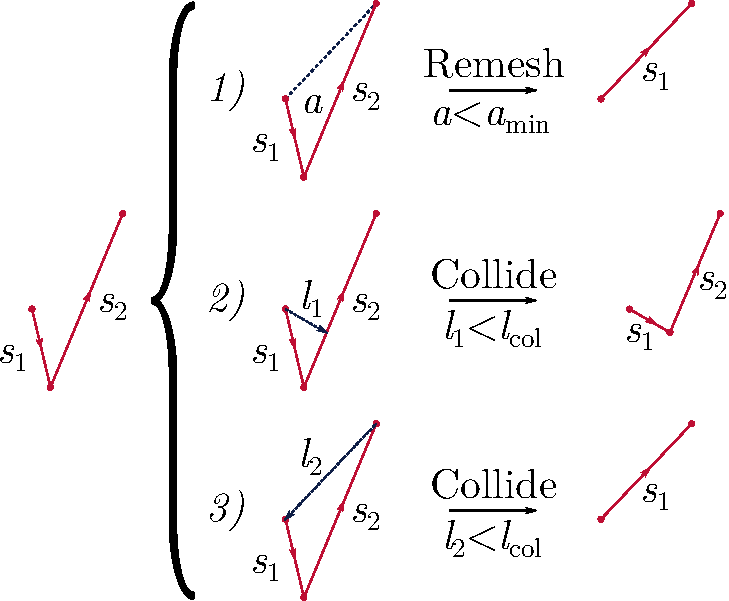
\includegraphics[width=0.7\linewidth]{hinge.pdf}
    \caption[A single dislocation hinge can lead to three different final topologies.]{A single dislocation hinge can lead to three final topologies (two of which are degenerate), the conditions for which can be simultaneously met in any combination. Where $a$ is the enclosed area, $l_1$ and $l_2$ are possible minimum lengths between both segments.}
    \label{f:hinge}
\end{figure}

The combination in which the conditions can be met, and the order in which they are checked could have drastic downstream consequences (see \cref{s:nonCommutativity}). \emph{Especially} at high dislocation densities where multiple collisions happen at every timestep. This had not been an issue prior to many of the improvements made to the codebase, but with the increased ability to model a larger number of dislocations to a sufficiently advanced point where this was having a significant impact, particularly in Haiyang Yu's nanoindentation simulations, which would either go wrong by creating unphysical junctions and/or massively slow down after reaching a certain point.

This was a multi-stage fix, where each fix progressively uncovered more and more shortcomings resulting from the unavoidable coupling between topological operations. These progressive fixes are detailed in \cref{s:nonCommutativity}. Here we will only focus on problems with collisions.

The first fix involved prioritising hinge collisions above the other type of collision, which we call \emph{two-line} collision. This meant detecting and resolving all possible hinge collisions before detecting and resolving any two-line collision. The rationale behind this is that segments in a hinge are already part of a single dislocation line. Because they are connected to each other at a single hinge node, they are already interacting via line tension and remote interaction; whereas two unconnected segments approaching one another only interact via remote interaction. The other, more practical advantage of resolving hinges first is that hinge collisions decrease the total segment length of the involved segments, therefore reducing their collision radii and the probability of them colliding with other segments via two-line collisions.

The second was much more subtle. \Cref{f:hinge} has two options for colliding a hinge, as seen in \cref{f:hinge}. Both resulting in different topologies. Which topology we ended up with was down to which segment, $s_1$ or $s_2$, the code came across first. If $s_1$ was first, then the answer would be $2)$, otherwise it would be $3)$. At the very least, the answer should be the same for a given network topology, regardless of how it is represented. So we decided to ensure the distance calculated was always the minimum out of both scenarios. Which means the distance calculated should be the minumum distance between the non-hinge node of the short segment, to the long segment. There is an argument to be made that the solution should be the other way round, as that would ensure the final structure has the minimum total length, as well as one less node. However, this could potentially leave many hinges around that would have otherwise been resolved.

\subsection{Collision distance}\label{ss:collisionDistance}

In the same vein as \cref{ss:hinges}, two-line collisions were being improperly prioritised. They occurred arbitrarily as the code came across them. Again yielding different answers for different representations of the same network. Only this time it had to do with the collision radius, as shown in \cref{f:collisionRadius}.
\begin{figure}
    \centering
    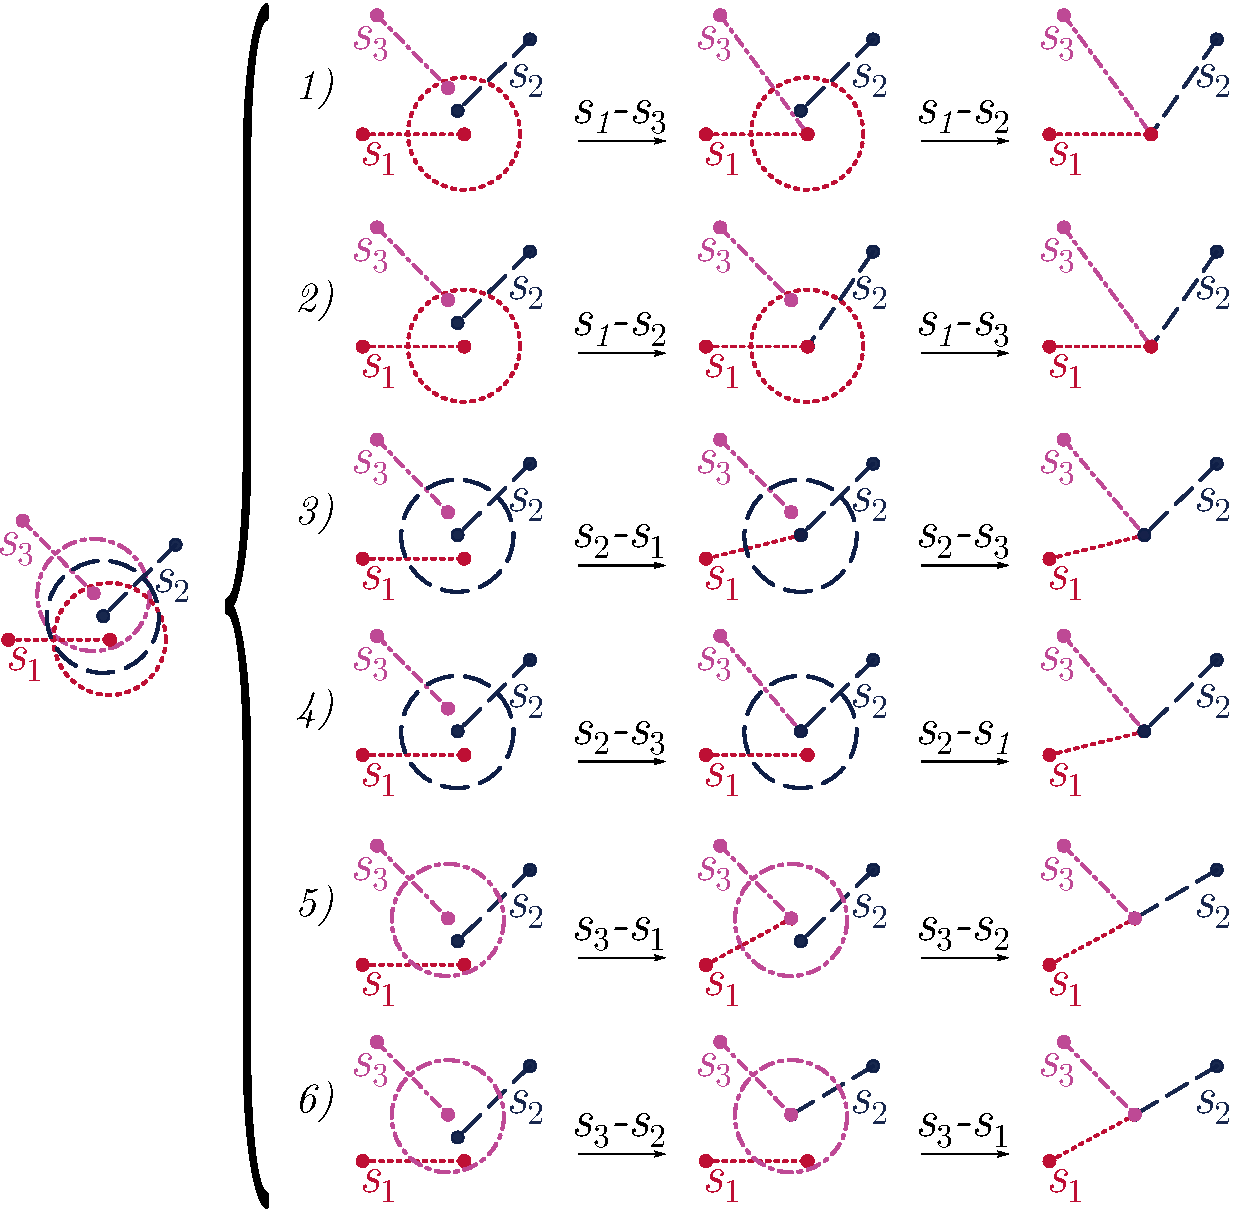
\includegraphics[width=0.9\linewidth]{collisionDist.pdf}
    \caption[Dislocation segments inside different collision radii.]{Multiple dislocation segments inside the same collision radius. Resolving all collisions at once leads to 3 different structures, 6 total but half are degenerate. Circles represent collision radii for the segments with corresponding line style and colour.}
    \label{f:collisionRadius}
\end{figure}

The actual algorithm is more sophisticated because it accounts for whole segments, as well as their relative velocities. It returns the points along the segments that minimise the distance between segments. These points are then used to decide which nodes and how they should be merged.

The problem was that as soon as a viable collision was found, the function returned. So in a scenario like \cref{f:collisionRadius}, if the code was looking for a collision on $s_1$, and it came across $s_3$ first, it would flag that as the collision, disregarding the fact that not only was $s_2$ closer, but $s_2$ and $s_3$ are also closer; and perhaps the true minimal distance was not even between $s_1$ and another segment, but between $s_2$ and $s_3$. We had to apply the same fix to hinge collisions. Admittedly, it matters less in that case as they tend to be rarer, plus their size is limited anyway, but still ensures a more correct solution.

The original algorithm had $\mathcal{O}(N^2)$, $\Theta(N^2/4)$ and $\Omega(N)$ for its upper, average, and lower bounds respectively for fixed $N$, where $N$ is the number of segments. The new one is always $\mathcal{O}(N^2)$. However, $N^2/4 \to N^2$ as $N\to\infty$, so as simulations grow larger, the performance hit gets lower. Moreover, the algorithm is quite cheap compared to other processes, and the improved accuracy is very much worth the small cost.

Better collision detection tends to result in faster simulations because the resulting structures are guaranteed to either produce the shortest segments---which can be cleaned up by remeshing---and therefore more accurate junctions. Referring back to \cref{f:collisionRadius}, it is evident that the structure formed by colliding $s_1$ and $s_3$ is higher energy than that formed by colliding $s_1$ and $s_2$. In this case, if we fully resolve the two possible collisions for every combination of segments, we arrive at three different scenarios (6 total but half are degenerate). However, this still leaves room for producing different answers given different representations of the network. If, for example the most appropriate collision is $s_2$-$s_3$ (cases 4 and 6 in \cref{f:collisionRadius}), the order in which it is performed can yield two slightly different structures after resolving the remaining collisions. However, this is preferrable over finding other, less favourable collisions that may lead to unecessarily complex structures.

We must also bear in mind that \cref{f:collisionRadius} shows a minimal example for a case where three collision radii overlap, and the resulting structures are not dissimilar to one another. In fact, if the final junction formed is glissile, they should evolve similarly. However, as the code was now able to handle and evolve larger numbers of dislocations further than before, it became apparent that the collision algorithms needed to be improved. After all, as the number of candidate collisions increased, so did the chance for the code to pick the wrong one and for that to have a deleterious effect on the code.

\section{Separation}

One of the larger problems with higher dislocation densities is the computational complexity of the separation function. Its role is to take high energy, highly connected structures and break them apart into lower energy, lower connection ones.

The separation criteria is the power dissipation of the split configuration compared to the power dissipation of the unseparated structure,
\begin{align}\label{eq:powerDiss}
    W_m & = \sum\limits_{i}\vec{v}_i \cdot \vec{f}_i\,,
\end{align}
where $W_m$ is the power dissipation of splitting mode $m$, $\vec{v}$ is nodal velocity, $\vec{f}$ nodal force and the sum over $i$ are the nodes participating in the splitting mode $m$. For the reference (pre-separation power dissipation), there is only one node involved in the calculation; the post-separation power dissipation involves the two nodes the node splits into. The splitting mode chosen by the separation subroutine is the one which dissipates the largest amount of power. If the pre-separation node has a higher power dissipation than any separation mode, it remains unseparated. In practice, the reference power dissipation is multiplied by a factor 1.05 to prevent nodes from flickering between being separated and colliding over multiple timesteps until the nodes move far enough apart that they can no longer collide.

Separation is a very poorly scaling operation,
\begin{align}
    \mathcal{O}\left(\sum\limits_{i}\sum\limits_{j=2}^{\left\lfloor C_i/2 \right\rfloor} \dfrac{C_i!}{(C_i-j)! j!}\right)\,.
\end{align}
Where the sum over $i$ is done over the nodes with more connections than is allowed; $C_i$ is the number of connections for node $i$; and $j$ is the number connections $C_i$ connections can be split into. Mirror symmetries where $2j = C_i$ half the number of possible splitting configurations for that case. At best, this puts the lower bound at approximately Sterling's factorial formula $N! \approx \mathcal{\Theta}(N\log{N})$ for large $N$. Furthermore, all of these configurations must be generated---an $\mathcal{O}(M)$ operation where $M$ are the number of nodes to be added---in order to check their power dissipation. Unfortunately, this is a relatively expensive operation because the code dynamically expands the relevant arrays. The nodal velocities and segment forces must then be calcualted for every configuration. Whichever configuration represents the and highest energy dissipation is picked as the final configuration. Locality is assumed, so only the forces and mobilities of the segments directly involved in the split are calculated. It is therefore extremely important that the number of separations each step be kept to a minimum.

The solution may appear to be as simple as calling separation after resolving a single collision, and looping through all collisions in a given timestep. However, this can cause collisions to be undone, leading to an infinite loop. If this happens, and there is no change in the number of nodes and links pre- and post-collision-separation, the offending segments are stored in a buffer whose entries are skipped by the collision detection. Once the segments have been added to the buffer, the iteration is run again without updating the network, and the collision detection will skip any pairs of colliding segments in the buffer. Once a successful collision-separation loop is performed, the buffers are deleted and the cycle repeats itself until there are no more collisions that cause the network to change. This means collisions can be checked more than once, but in keeping with the quasi-static conditions, ensures all first-order\footnote{A true minimal energy structure would require all collisions to be performed and a full traversal of every splitting mode tree.} energetically favourable topological operations are performed every timestep while preventing infinite loops. This, together with the fixes made to the collision detection, ensures subsequent iterations of the collision-separation loop utilise minimal energy structures. An added benefit is that it also keeps the number of possible separations to a minimum because single collisions get resolved every iteration.

It is worth noting that nodes labelled as immobile (an artificial construct to mimic pinning) are not split by separation. Which means they sometimes become very highly connected and as a result can create an impassable obstacle for other nodes. As a result, they get `unpinned' when they reach a critical level of connectivity. Separation is performed after this check to break them apart, and also because nodes may need separating despite there being no collisions during the timestep.

The role of remeshing is to ensure the resolution of the network is appropriate. It does so by ensuring there is an appropriate number and distribution of nodes throughout the network to keep discretisation accuracy high, whilst minimising computational cost. Therefore, the final piece of the puzzle was remeshing the network pre- and post-collision-separation loop, so the next iteration starts with a clean network.

\section{Non-commutativity of topological changes}\label{s:nonCommutativity}

For a given iteration, the time-evolution and topological changes were performed in the following order:
\begin{enumerate}
    \item time-evolution,
    \item separate highly connected nodes,
    \item detect and resolve collisions, and
    \item remesh network.
\end{enumerate}
This ordering is problematic. Fundamentally, this means the time evolution erroneously accounts for complex structures that should have dissipated into lower energy ones as per the quasi-static principle our model is based on. In other words, detecting and resolving collisions, generates highly connected structures that are high energy and thus produce large local stress gradients. The assumption that a node and its neighbours experience similar conditions breaks down near these highly connected nodes. Moreover, the assmumption that the network is at thermodynamic equilibrium at every time step breaks down when there are highly connected nodes that otherwise be broken up by separation. Both of these lead to \cref{eq:nodeVel} not holding, which is the fundamental assumption behind our mobility laws.

Moreover, the order in which topological changes were carried out was also very sub-optimal. Colliding after separating would result in nodes being separated only to immediately collide again. Remeshing only at the end also meant the input network for separation may contain segments that were either larger or smaller than the minimum allowable length. Meaning the network was not properly discretised before separations and collisions were performed, leading to incorrect structures. The solution to this problem is to also remesh the network after evolving it in time, ensuring the separation and collision subroutines were fed an appropriately discretised network.

The new order of operations, accounting for the improvements in collision and separation previously described is as follows:
\begin{enumerate}
    \item time-evolution,
    \item remesh,
    \item collision-separation loop,
    \item mobilise highly connected immobile nodes,
    \item separate highly connected nodes,
    \item remesh.
\end{enumerate}
This ensures the time evolution and topological functions are all fed a network that is as clean and well-resolved as the input parameters say it should be. Although this incurs a computational cost, the benefits of having a cleaner network for the other functions to work with vastly outweigh the increased cost of calling the cheap remeshing subroutine more times.

\section{Conclusions}

Discrete dislocation dynamics is a stiff and chaotic dynamical system. It is very sensitive to small changes, as we will see in \cref{c:tractions}. Having a correct topology is of the utmost importance in this regard. Something as small as a collision that was not performed when it should have, can have dramatic downstream consequences. As dislocation density increases, the degree of correctness when resolving their interactions increases in importance. Not only does it increase the accuracy of a simulation, but improves its running speed.

The increase in accuracy is obvious; detecting all the collsions that should be detected; resolving them in a manner more keeping with the quasi-static assumption yielding the mobility law; and ensuring the network resolution is what it should be; make for more accurate simulations.

Part of the increase in running speed is down to the fact that quasi-static conditions are better met than before, so the timsetep can be greater. The other huge benefit to running speed is down to the asymptotic scaling and high proportionality constant of the algorithms we use; $\mathcal{O}(N^2)$ for seg-seg forces and collisions; $\mathcal{O}(C_i!)$ for a single separation; $\mathcal{O}(M N)$ for tractions. Where $N$ is the number of segments, $C_i$ the number of connections, and $M$ the number of surface elements. Simply put, the fewer things to calculate have a disproportionately large impact on how many operations need to be performed every time any of these functions is run.

With these improvements, simulations that used to be computationally intractible within a reasonable timeframe are now very doable. Large, complex simulations with high dislocation densities are still slow by virtue of how topologically active they are. They are simultaneously more accurate and faster by multiple orders of magnitude (sometimes 5 or more) than before.
\savearabiccounter
%2366 words